\documentclass{article}
\usepackage{palatino}
\usepackage{graphicx}
\usepackage{listings}
\begin{document}

\title{Senior Project: GPU Computing}
\author{John Kloosterman \\
  \texttt{john.kloosterman@gmail.com}}
\date{September 2012-May 2013}
\maketitle



\section{Test Computer}
Using funds from one of Prof. Adams' NSF grants, I built a system for testing GPU programs. This system included four different devices that OpenCL supports: the CPU, the small Intel GPU integrated into the processor, an AMD Radeon 7970 GPU, and two nVidia GTX 480 GPUs.

The theoretical peak performance of this system is XXX TFLOPS. This is comparable to Dahl, Calvin's supercomputer, which has a theoretical peak performance of XXX TFLOPS. 

This system was used for all benchmarks in this report. The CPU used is an Intel Core i7-3770, and the GPU used for benchmarks is the AMD Radeon 7970.

\section{OpenCL Framework}
OpenCL is designed to be flexible, but this means that it is unwieldly for developers to use. The simplest OpenCL program that runs code on a GPU is [[[]] lines long. The framework is an attempt at making OpenCL kernel calls syntactially as similar as possible to calling a C++ function or method.

\subsection{Functions vs. Kernels}
The entry point of an OpenCL program is a kernel, marked with the \texttt{\_\_kernel} keyword. This framework wraps around OpenCL's native functionality with the CLKernel class, making it simpler to compile kernels, pass parameters to them, and set the local and global workgroup size of the kernel. An example usage of the CLKernel class is [FILE NAME].

OpenCL does not support calling non-kernel functions, but these functions need some way to be tested. The \\texttt{CLFunction} class in this framework removes OpenCL's limitation. A kernel to call the function is automatically generated at compile-time, and that kernel is passed to OpenCL. \texttt{CLFunction} will run the function on one thread.

More complex functions, especially those that involve threads cooperating on a task with data stored in local memory, cannot be called by \texttt{CLFunction}. One idiom I developed when testing these kinds of functions, is to write a shim kernel that copies data into the correct memory space, calls the function to be tested, then copies the results back to \texttt{\_\_global} memory. (See [FILE NAME] for an example)

\subsection{Usage}
C++11 constructs allow a class to syntactically behave like a variadic function, by defining an overloaded () operator using a variadic template. At this time, compilers only partically support the features needed to make using variadic templates elegant. With C++11, a \texttt{CLKernel} or \texttt{CLFunction} can be called like this:

\begin{lstlisting}
#include <CLKernel.h>

string src; // some kernel source code
cl_int i, j, k;
CLKernel theKernel( ''kernel_name'', src );
theKernel( i, j, k );
\end{lstlisting}

Microsoft Visual Studio 2008 (the version that AMD's OpenCL tools currently target) does not support C++11. This requires a clunkier syntax:

The CLUnitArgument class has constructors for many different types, which means that variables of those types can be passed into a CLKernel or a CLFunction without needing to explicitly create a CLUnitArgument.

\subsection{Other Features}
I found I was often developing on my laptop, which does not have an OpenCL-supported GPU. The framework automatically degrades to using a CPU if there are no GPUs, so that programs will still run, albeit much more slowly in most cases.

If the \texttt{CL\_DEBUG} environment variable is set to 1, the framework will compile kernels with debugging symbols and run them on the CPU. This allows for debugging kernels using gdb as described in the AMD OpenCL guide (reference).

\section{Raytracer}
As a simple application to run on top of my framework, I implemented an OpenCL raytracer for honours credit in CS 352 (Computer Graphics). The raytracer maps one pixel onto one hardware thread.

\subsection{Capabilities}
The raytracer has two geometric primitives: spheres and planes. Geometry can have a colour or be reflective. There can be any number of geometric primitives.

The lighting model takes into account ambient and diffuse lighting. There can be any number of diffuse light sources.

\subsection{Limitations}
Because OpenCL does not support recursion, reflective surfaces do not behave as they do in other raytracers. Reflective surfaces shoot a ray off the reflective surface, and the ray takes the colour of the first object it hits, taking into account only ambient lighting (see Figure \ref{fig:reflections}). Other raytracers are able to take into account other types of lighting from the reflected surface, and can simulate rays being reflected more than once. This is not possible with this implementation, because it would involve a recursive call from the lighting function to the lighting function.

\begin{figure}[ht!]
\centering
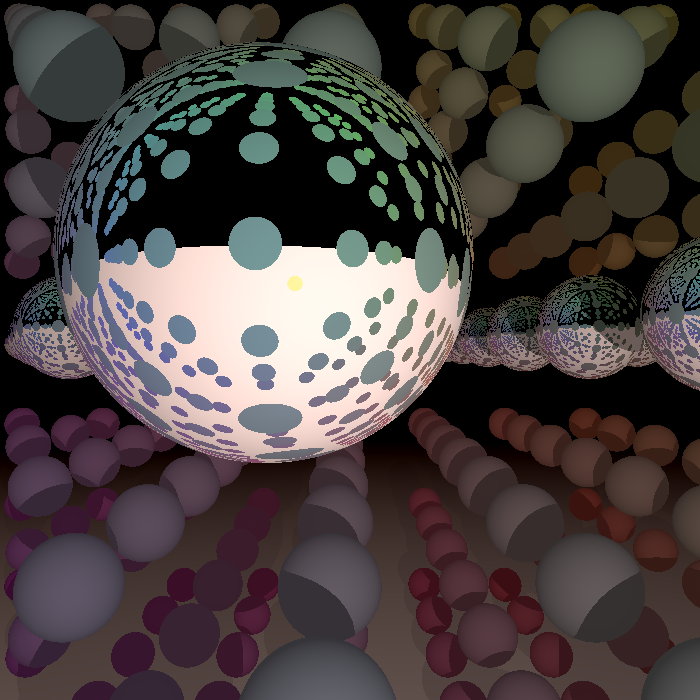
\includegraphics[width=90mm]{reflections.png}
\caption{Reflections that only take into account ambient lighting}
\label{fig:reflections}
\end{figure}

\subsection{Performance}
The raytracer is able to render a 700x700 pixel test scene with 1000 spheres and a moveable diffuse light source at speeds that make it interactive (see figure \ref{fig:testscene}). Using the CPU, this scene takes 1.28 seconds per frame (0.78 frames per second). Using the Radeon 7970, the scene takes 0.055 seconds per frame (18 frames per second). If the number of spheres is reduced to 216, the Radeon 7970 can render the scene at 60 frames per second.

\begin{figure}[ht!]
\centering
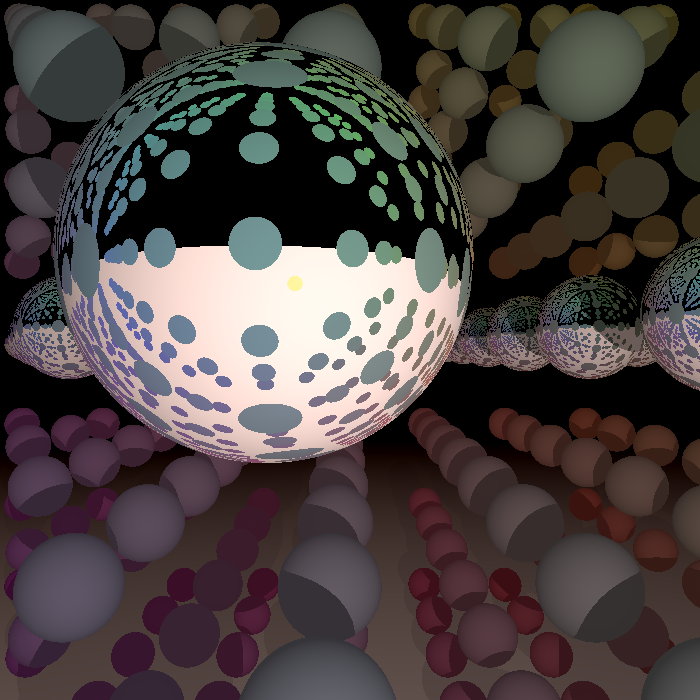
\includegraphics[width=90mm]{reflections.png}
\caption{Test scene with 1000 spheres and ground plane}
\label{fig:testscene}
\end{figure}

\section{Mankalah Minimax AI}
This part of the project implemented a minimax player for the Mankalah game introduced in CS 212. Minimax is a much harder algorithm to implement on a GPU than a raytracer, because the minimax tree has dependencies between nodes, and the parallelism is less obvious.

\subsection{Strategy}
Following REFERENCE, the minimax tree is broken up into layers. On the CPU, the first layers of game boards in the minimax tree are computed and the bottom-level leaf nodes of that tree are put into a C++ vector. The boards in the vector are copied over to the GPU, where 4 more levels of minimax are computed. Because the Mankalah minimax tree has a branching factor of 6, the overwhelming majority of the work is done in the bottom 4 levels of the tree.

INSERT DIAGRAM FROM REFERENCE

\subsection{Performance}



\section{Economics Simulation}


\section{\_\_local Memory malloc()}


\end{document}
